\section{Protocolo de comunicação}

Esta seção detalha o protocolo de comunicação estabelecido entre a estação base, a placa TS-7260 (sistema com linux embarcado) e a placa LPC2103 (sistema embarcado de baixo nível).

O protocolo desenvolvido para a comunicação (via Wi-Fi) entre a estação base e a TS-7260 visa utilizar o TCP como camada de transporte. Como foi explicitado anteriormente na seção \ref{subsec:pacote_comunicacao}, o robô foi escolhido como servidor da conexão, e a estação base como cliente. Para haver confirmação da conexão entre os dois, optou-se por criar um protocolo de \textit{handshake} semelhante ao existente no TCP, de 3 passos: requisição, resposta, confirmação. A requisição é feita pelo cliente no início da conexão, a resposta é dada pelo servidor em seguida. Posteriormente, o cliente envia uma mensagem de confirmação, e a conexão é totalmente estabelecida. O uso do \textit{handshake} contribui para tanto a estação base como o sistema embarcado confirmarem que estão conectados um ao outro e não a um servidor/cliente qualquer.

Para possibilitar que o tráfego de mensagens possa ser feito de forma rápida, reduzindo atrasos, o envio e recebimento de mensagens é feito de forma assíncrona.
Essa escolha foi feita tendo em vista que, em uma comunicação totalmente síncrona, um programa (ou thread) é bloqueado ao chamar uma função de recebimento ou envio, até que efetivamente seja completa a transação. Supondo que só houvesse uma thread gerenciando a conexão, o programa não poderia enviar ou receber dados ao mesmo tempo em \textit{full-duplex}, mas somente \textit{half-duplex} (somente enviar ou somente receber).

A solução desenvolvida para possibilitar a comunicação assíncrona foi o uso de 4 threads (tanto na estação base quanto no sistema embarcado) para gerenciar os diversos aspectos envolvidos nela. A primeira \textit{thread} (a gerenciadora principal de conexão) é a responsável por estabelecer e manter a conexão, além de gerenciar os potenciais erros que possam ocorrer (tempo excessivo sem comunicação e fechamento de socket). Para a estação base, o diagrama de estados dessa \textit{thread} está representado na Figura \ref{fig:diagrama_estados_estacao_base}, e para o sistema embarcado na Figura \ref{fig:diagrama_estados_sist_embarcado}.

A segunda \textit{thread} tem a função de gerenciar o envio de mensagens. O programa principal, ao necessitar enviar uma mensagem, faz uma requisição a essa \textit{thread} que insere a mensagem em uma fila de envio. O programa principal não fica bloqueado, dessa forma, pois não necessita aguardar a mensagem ser completamente enviada, podendo efetuar outras tarefas. O diagrama de estados dessa \textit{thread} está presente na Figura \ref{fig:diagrama_estados_sender}.

A terceira \textit{thread} gerencia o recebimento de mensagens. Seu funcionamento é relativamente simples: ela possui um loop, no qual aguarda até alguma mensagem ser recebida. Quando ocorre o recebimento de alguma mensagem, ela é encaminhada para a quarta \textit{thread} (cuja explicação está a seguir) que processa o conteúdo dela e executa as operações que são necessárias para cada tipo de mensagem. Dessa forma, novas mensagens podem ser recebidas rapidamente, pois o receptor não fica bloqueado realizando o processamento das informações recebidas. O diagrama de estados dessa terceira \textit{thread} está presente na Figura \ref{fig:diagrama_estados_receiver}.

A quarta \textit{thread}, como já exposto, é a responsável por processar mensagens recebidas e realizar as operações que são necessárias para cada tipo de mensagem, o que depende da codificação exposta na seção \ref{sec:codificacao_mensagens}. Ela possui uma fila, na qual são inseridas as mensagens a serem processadas. Dessa forma a \textit{thread} receptora não necessita ficar bloqueada aguardando o término do processamento. O diagrama de estados dessa quarta \textit{thread} está presente na Figura \ref{fig:diagrama_estados_processor}.

\subsection{Diagramas de estados}

Nesta seção estão expostos os diagramas de estados do protocolo de comunicação nas Figuras \ref{fig:diagrama_estados_estacao_base}, \ref{fig:diagrama_estados_sist_embarcado}, \ref{fig:diagrama_estados_sender}, \ref{fig:diagrama_estados_receiver}, \ref{fig:diagrama_estados_processor} e \ref{fig:diagrama_estados_amostragem_sensores}.

Um aspecto importante a ressaltar é que, nas \textit{threads} de envio (Figura \ref{fig:diagrama_estados_sender}) e de processamento de mensagens (Figura \ref{fig:diagrama_estados_processor}), pode haver adição assíncrona de elementos na fila. Ou seja, quando é feita a verificação do número de elementos presentes na fila (como representado nos diagramas), tem-se em vista que elementos podem ter sido adicionados a qualquer instante. Obviamente, no ponto de vista da implementação, existem as seções críticas que devem ser devidamente gerenciadas para evitar condições de disputa e outros problemas de concorrência. Porém, as seções críticas se resumem aos acessos à fila somente, o que reduz consideravelmente a complexidade do processo.

Na Figura \ref{fig:diagrama_estados_amostragem_sensores} está exposto o diagrama de estados da \textit{thread} do sistema embarcado que é responsável por realizar a amostragem dos sensores em intervalos fixos de tempo. Ela realiza a amostragem enviando periodicamente -- quando programada -- comandos SYNC (vide seção \ref{sec:codificacao_mensagens}) para a placa de baixo nível. Vale ressaltar que para melhor explicar este processo, na Figura \ref{fig:diagrama_sequencia_motores} da próxima seção está exposto um diagrama de sequência que demonstra a amostragem dos sensores.



\begin{figure}[H]
  \centering
  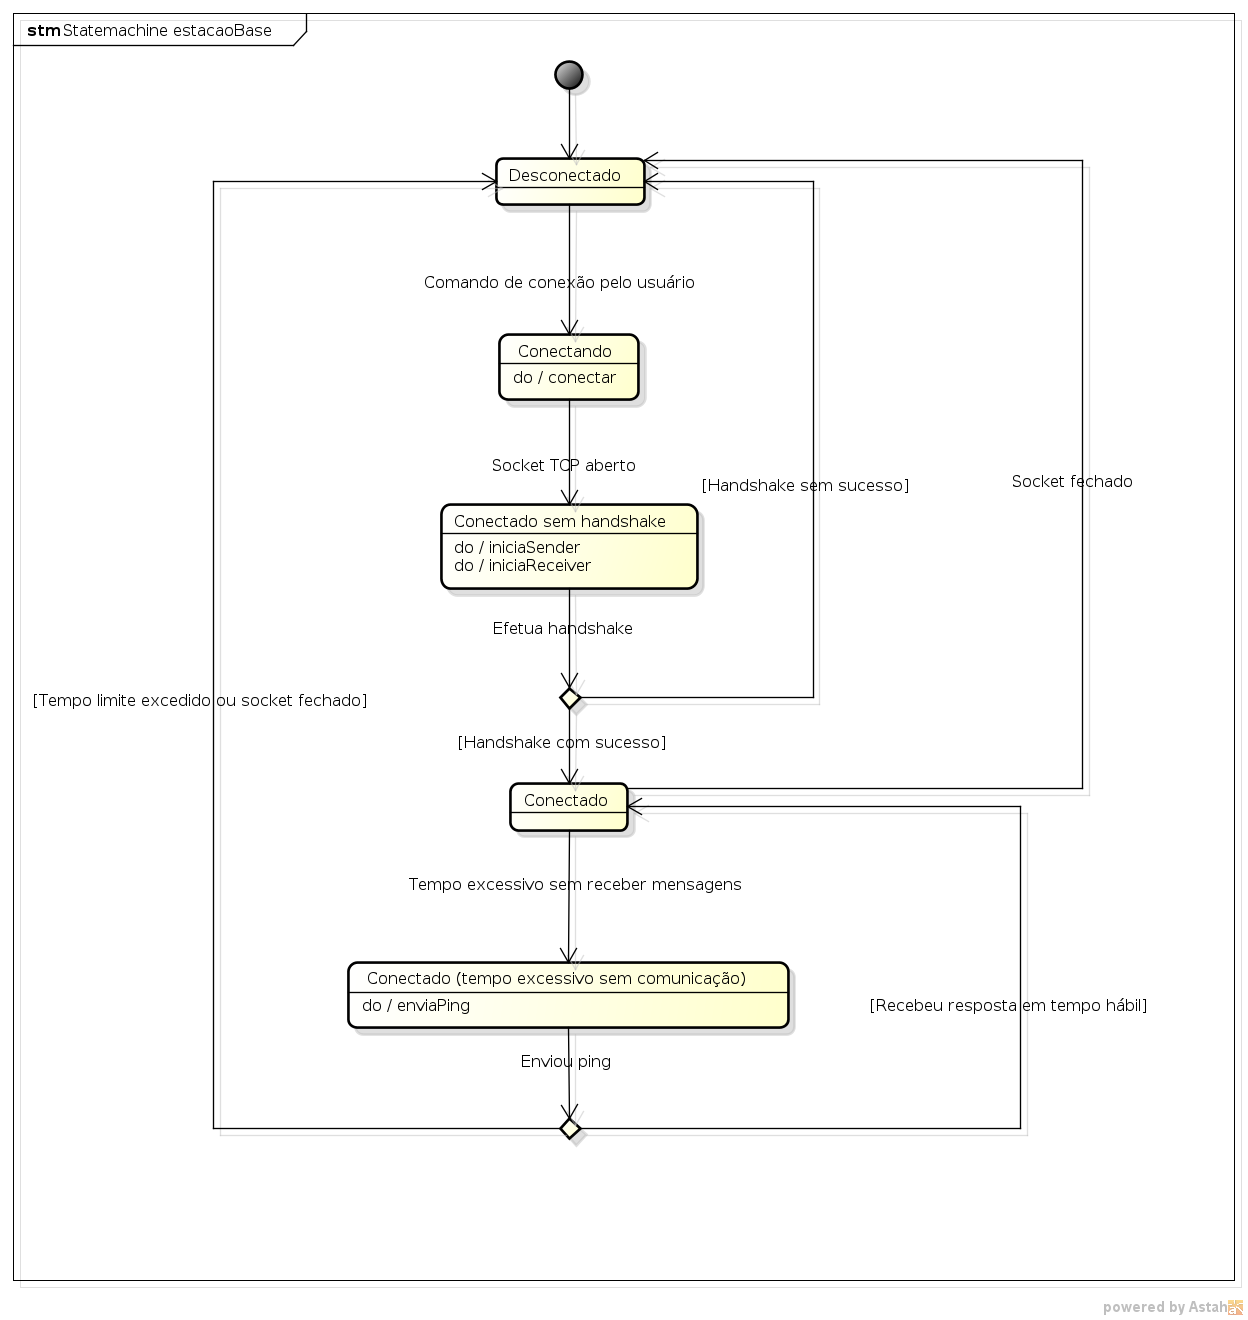
\includegraphics[width=\textwidth, keepaspectratio]{./figuras/diagrama_estados_estacao_base.png}
  \caption{Diagrama estados da \textit{thread} principal da conexão da estação base.}
  \label{fig:diagrama_estados_estacao_base}
\end{figure}

\begin{figure}[H]
  \centering
  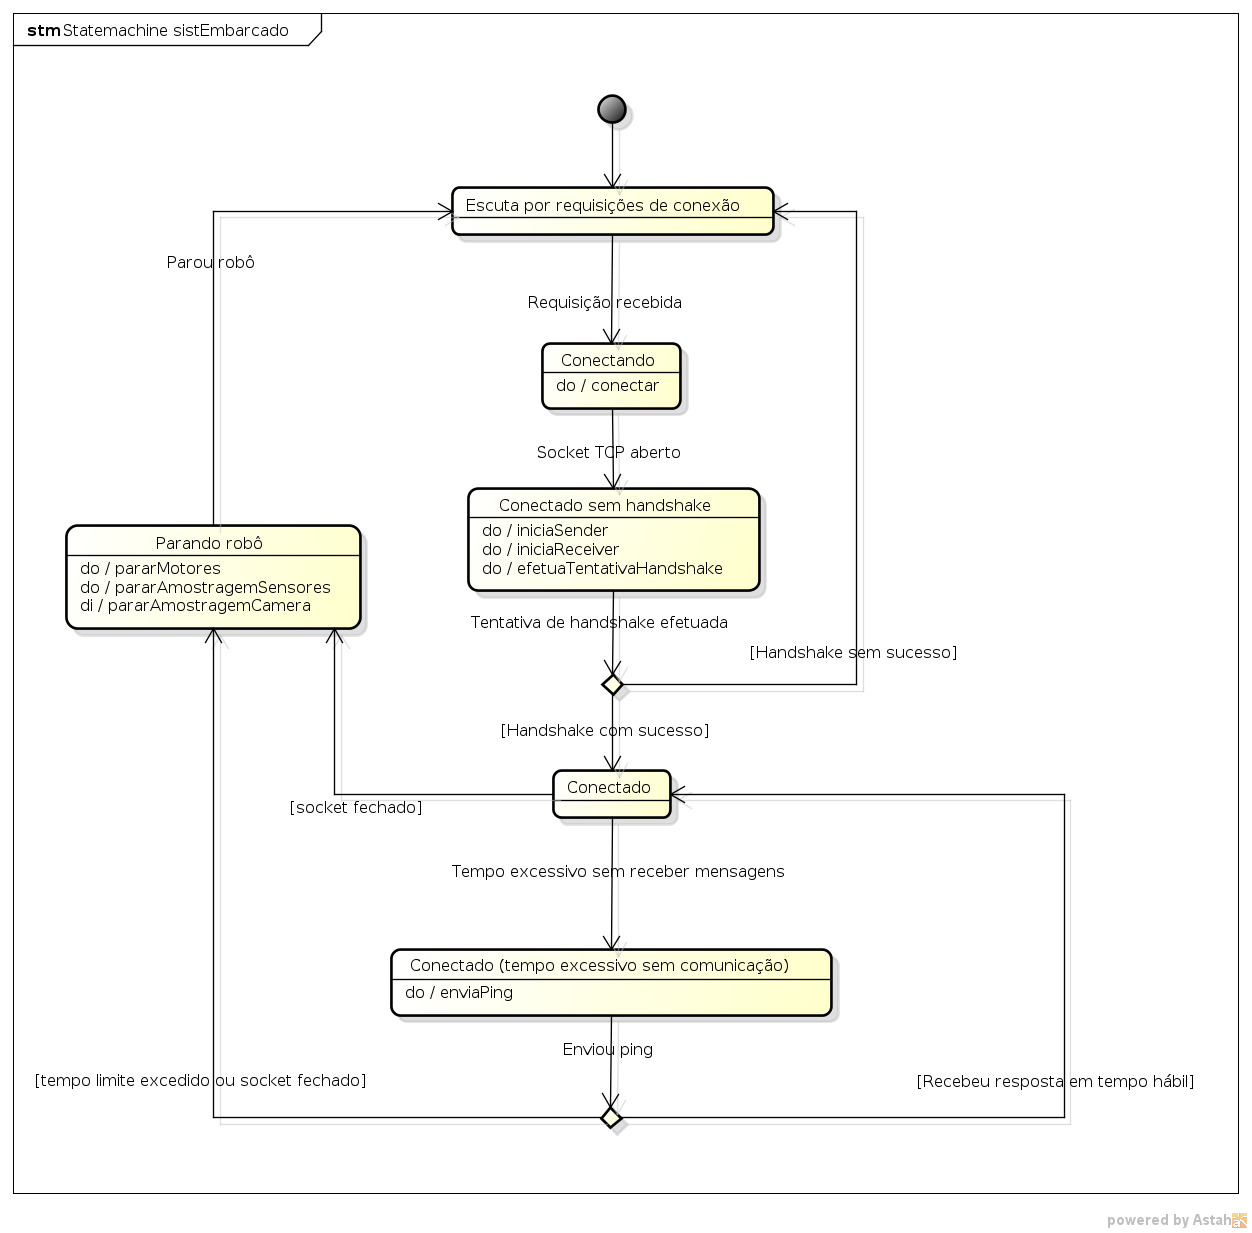
\includegraphics[width=\textwidth, keepaspectratio]{./figuras/diagrama_estados_sist_embarcado.png}
  \caption{Diagrama de estados da \textit{thread} principal da conexão do sistema embarcado.}
  \label{fig:diagrama_estados_sist_embarcado}
\end{figure}

\begin{figure}[H]
  \centering
  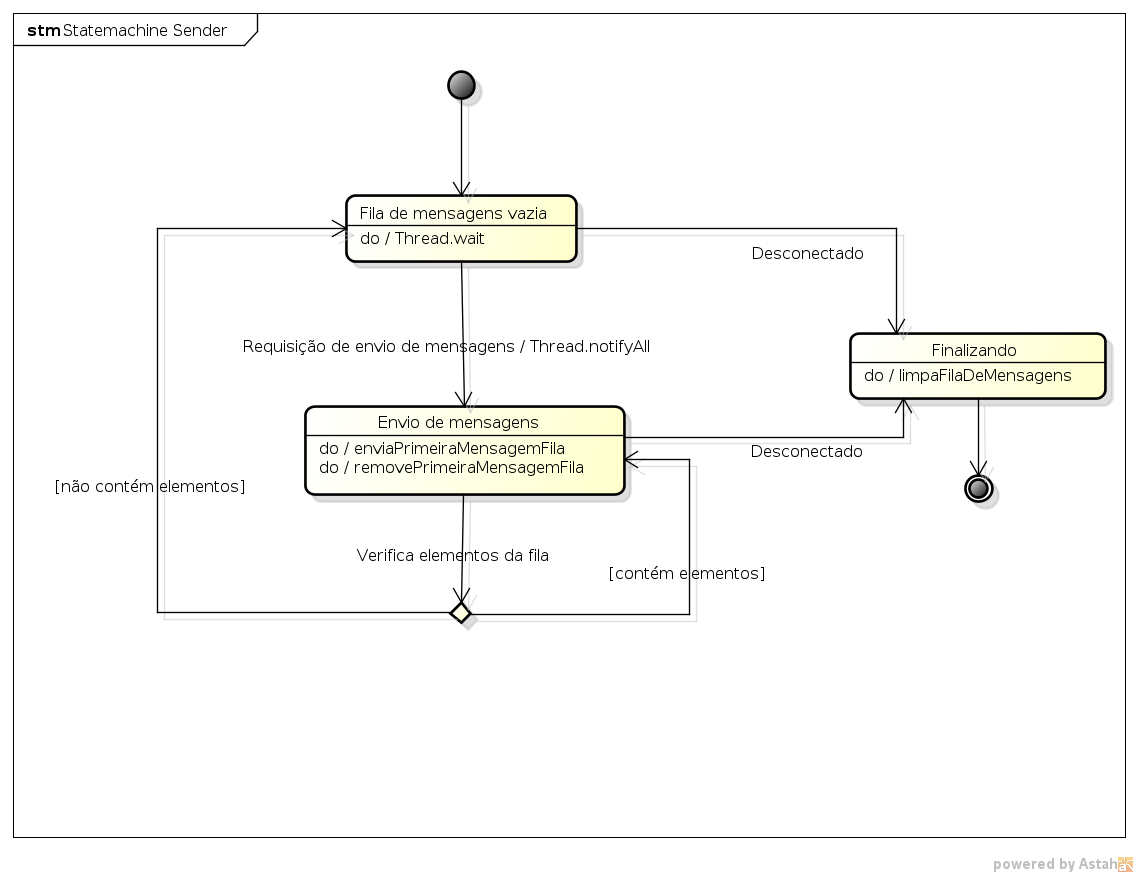
\includegraphics[width=\textwidth, keepaspectratio]{./figuras/diagrama_estados_sender.png}
  \caption{Diagrama de estados da \textit{thread} que envia mensagens (igual para estação base e sistema embarcado).}
  \label{fig:diagrama_estados_sender}
\end{figure}

\begin{figure}[H]
  \centering
  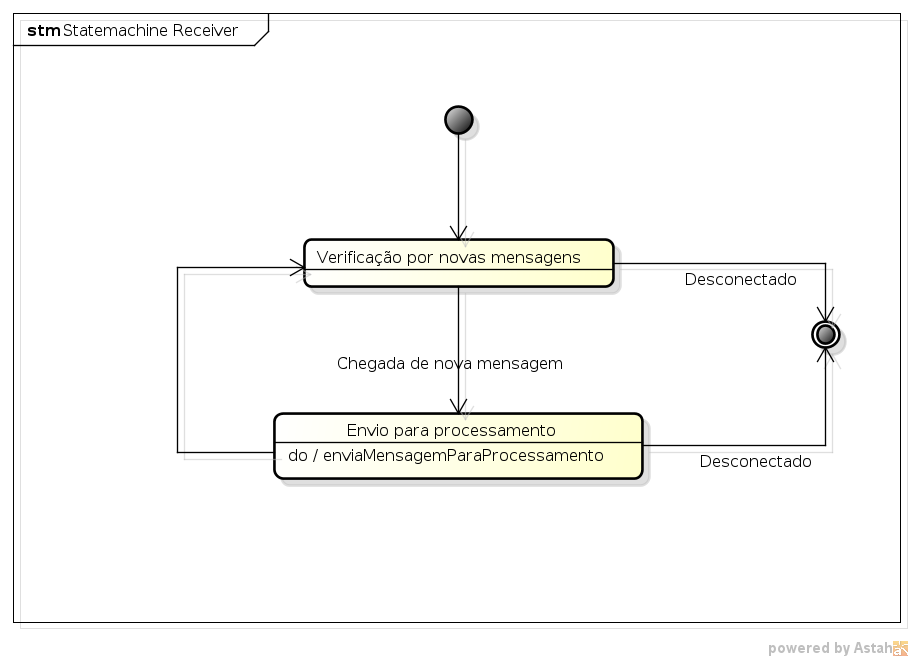
\includegraphics[width=\textwidth, keepaspectratio]{./figuras/diagrama_estados_receiver.png}
  \caption{Diagrama de estados da \textit{thread} receptora de mensagens (igual para estação base e sistema embarcado).}
  \label{fig:diagrama_estados_receiver}
\end{figure}

\begin{figure}[H]
  \centering
  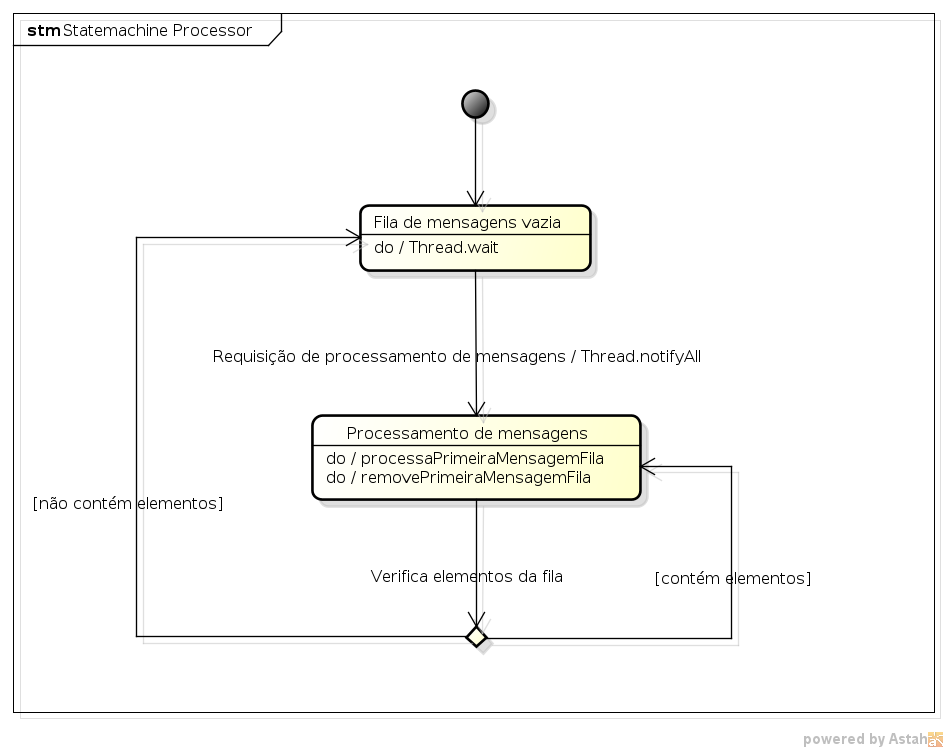
\includegraphics[width=\textwidth, keepaspectratio]{./figuras/diagrama_estados_processor.png}
  \caption{Diagrama de estados da \textit{thread} que processa mensagens recebidas (igual para estação base e sistema embarcado).}
  \label{fig:diagrama_estados_processor}
\end{figure}

\begin{figure}[H]
  \centering
  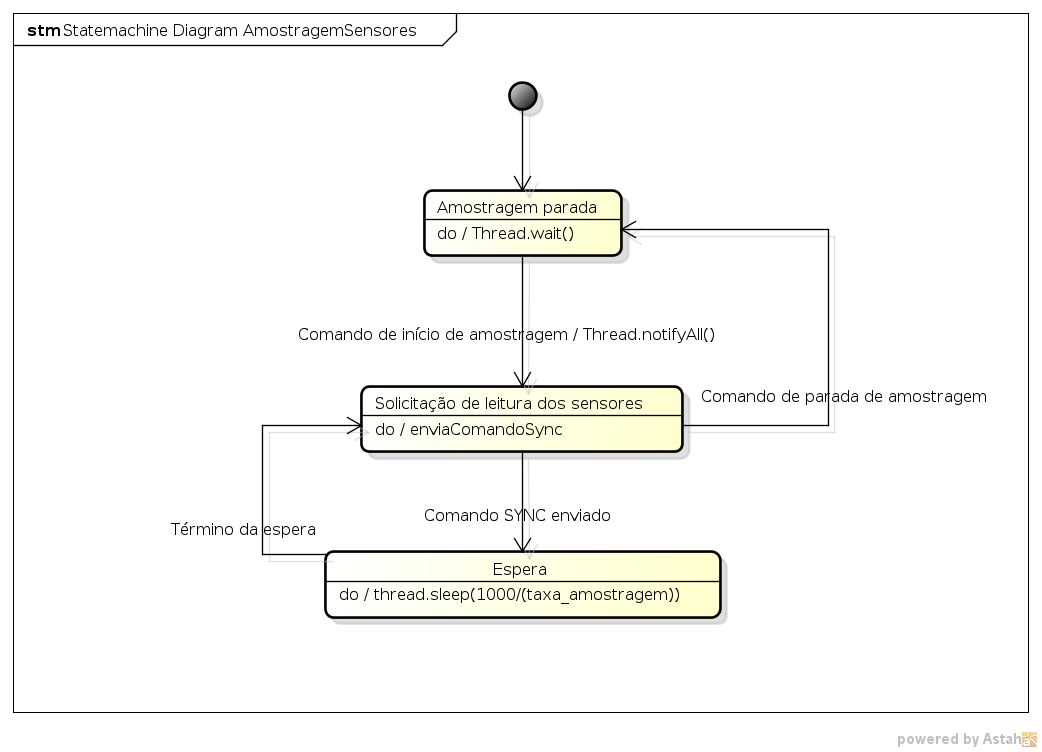
\includegraphics[width=\textwidth, keepaspectratio]{./figuras/diagrama_estados_amostragem_sensores.png}
  \caption{Diagrama de estados da \textit{thread} responsável por efetuar a amostragem dos sensores (sistema embarcado).}
  \label{fig:diagrama_estados_amostragem_sensores}
\end{figure}



\subsection{Diagramas de sequência}

Nessa seção estão presentes as versões iniciais de dois diagramas de sequência. O primeiro (Figura \ref{fig:diagrama_sequencia_motores}) representa como um comando de mudança de velocidade das rodas dado pelo usuário chega até a placa de baixo nível. O segundo (Figura \ref{fig:diagrama_sequencia_sensores}) demonstra a sequência dos dados de leituras dos sensores que saem da placa de baixo nível e chegam até o usuário. 

Vale ressaltar que as chamadas assíncronas, ou seja, que não bloqueiam a execução da \textit{thread} chamadora, foram representadas também nestes diagramas.

\begin{figure}[H]
  \centering
  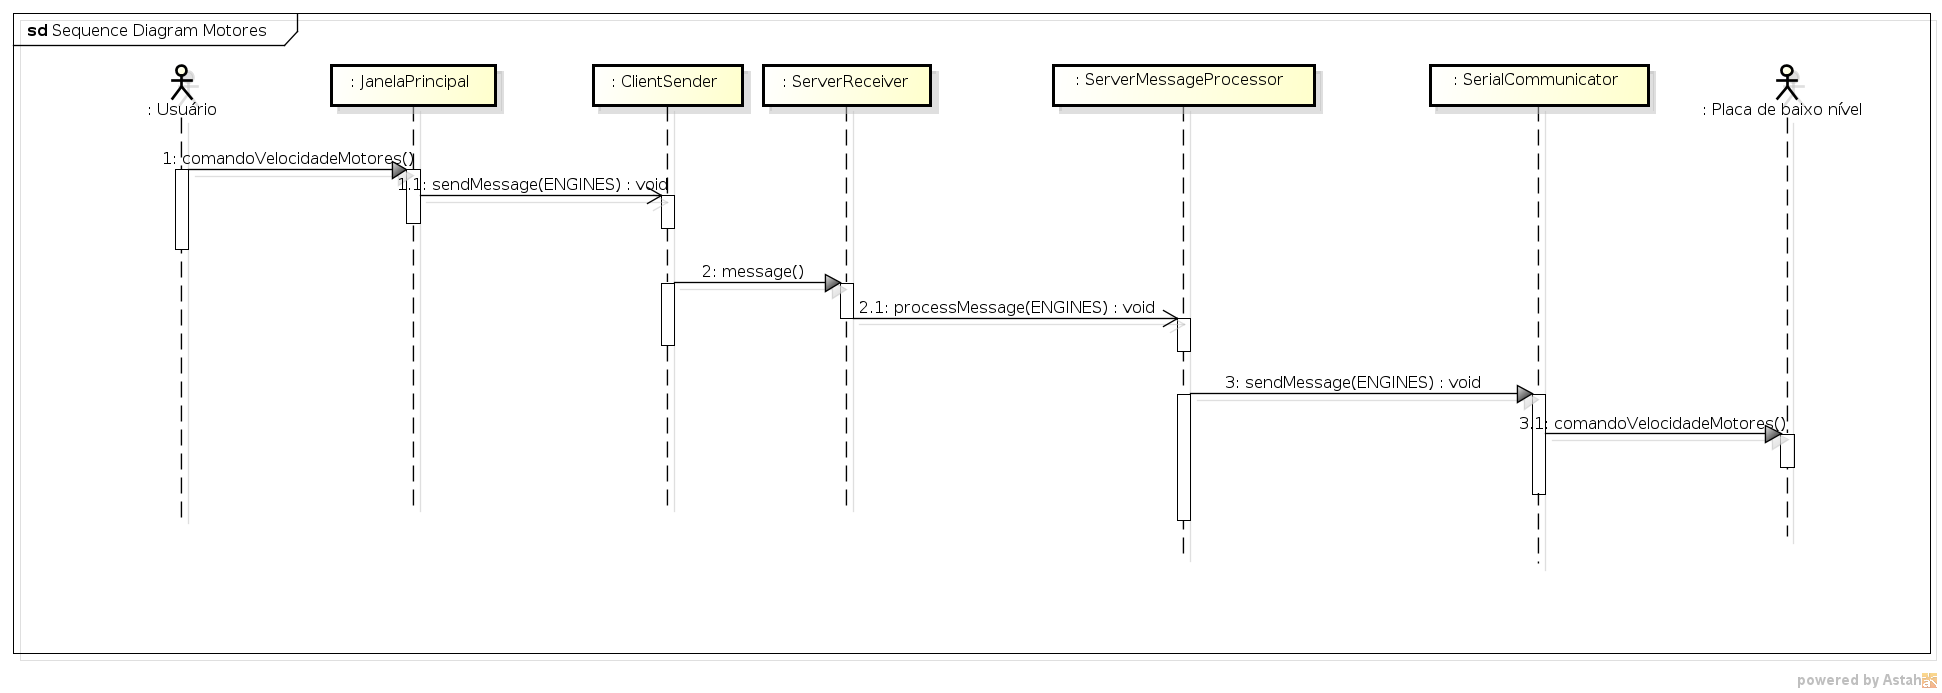
\includegraphics[width=\textwidth, keepaspectratio]{./figuras/diagrama_sequencia_motores.png}
  \caption{Diagrama de sequência de comando para mudança de velocidade dos motores.}
  \label{fig:diagrama_sequencia_motores}
\end{figure}

\begin{figure}[H]
  \centering
  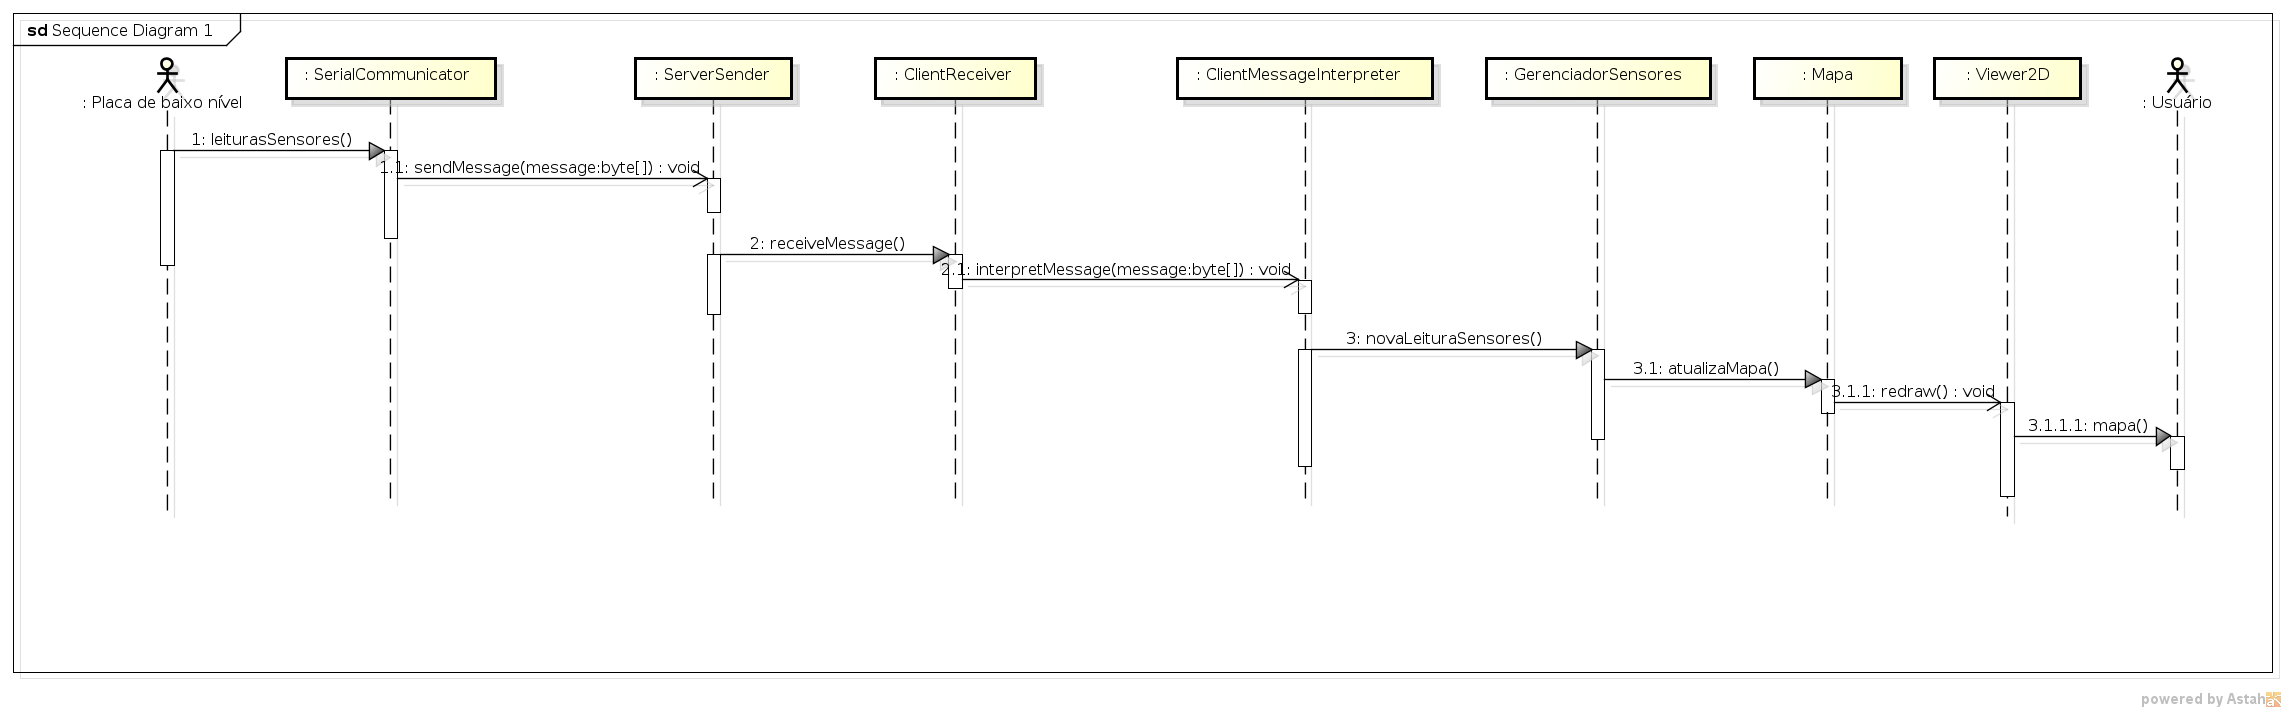
\includegraphics[width=\textwidth, keepaspectratio]{./figuras/diagrama_sequencia_sensores.png}
  \caption{Diagrama de sequência da amostragem dos sensores.}
  \label{fig:diagrama_sequencia_sensores}
\end{figure}


\subsection{Codificação das mensagens}
\label{sec:codificacao_mensagens}

\begin{itemize}
  \item Mensagens do TS-7260 para o LPC2103 (via porta serial)
  
	\begin{itemize}
		
	  \item \textbf{SYNC}\\
	  \textit{(byte) END\_CMD}\\
	  Quando o microcontrolador LPC2103 recebe esta mensagem, responde com as leituras mais recentes dos encoders, de cada sensor de distância, do acelerômetro e do giroscópio (enviando uma mensagem SENSORS, explicada abaixo).
	  
	  \item \textbf{ENGINES}\\
	  \textit{(byte) vel\_roda\_esquerda}\\
	  \textit{(byte) vel\_roda\_direita}\\
	  \textit{(byte) END\_CMD}\\
	  Ao receber este comando, o microcontrolador utiliza os valores para definir o nível de PWM para as rodas do robô. Os valores de velocidade são representados por um byte cada, nos quais o bit mais significativo indica o sentido de rotação da roda e os restantes a intensidade do PWM.
	  
	  \end{itemize}
	  
	  \item Mensagens do LPC2103 para a TS-7260 (via porta serial)
	  
	  \begin{itemize}
	  
	  \item \textbf{SENSORS}\\
	  \textit{(byte) encoder\_esq\_H}, \textit{(byte) encoder\_esq\_L},\\
	  \textit{(byte) encoder\_dir\_H}, \textit{(byte) encoder\_dir\_L},\\
	  \textit{(byte) IR1}, \textit{(byte) IR2}, \textit{(byte) IR3}, \textit{(byte) IR4}, \textit{(byte) IR5},\\
	  \textit{(byte) AX\_H}, \textit{(byte) AX\_L},\\
	  \textit{(byte) AY\_H}, \textit{(byte) AY\_L},\\
	  \textit{(byte) AZ\_H}, \textit{(byte) AZ\_L},\\
	  \textit{(byte) GX\_H}, \textit{(byte) GX\_L},\\
	  \textit{(byte) GY\_H}, \textit{(byte) GY\_L},\\
	  \textit{(byte) GZ\_H}, \textit{(byte) GZ\_L},\\
	  \textit{(byte) TIMESTAMP\_H}, \textit{(byte) TIMESTAMP\_L}\\
	  \textit{(byte) END\_CMD}\\
	  Representa a leitura de todos os sensores (encoders, infra-vermelhos, acelerômetro e giroscópio). 
	  
	  Os 4 primeiros bytes são os valores das leituras dos encoders esquerdo e direíto (cada um com um byte alto e um baixo). Os valores das leituras dos encoders representam a diferença entre a contagem atual a contagem anterior.
	  
	  Nos próximos 5 bytes, as leituras do sensores ópticos são enviadas em sequência. As distâncias que os sensores ópticos são capazes de mensurar são dividos em valores discretos de 0 a 255 \cite{bellator_2012}. 
	  
	  Após isso, os 12 bytes que se seguem representam as leituras do acelerômetro e do giroscópio. Os bytes que começam com `A' representam a leitura de cada um dos eixos do acelerômetro. Aqueles que começam com `G' representam a leitura de cada um dos eixos do giroscópio.
	  
	  O timestamp (valor alto e baixo) é um contador de 16 bits que zera automaticamente quando chega ao valor máximo, usado para controlar a perda e ordem dos dados.
	  
	  
	\end{itemize}

  \item Mensagens bidirecionais entre estação base e TS-7260 (via Wi-Fi):

    \begin{itemize}
      \item \textbf{ECHO\_REQUEST}\\
      \textit{(byte) END\_CMD}\\
	Requisição de ping.
      \item \textbf{ECHO\_REPLY}\\
      \textit{(byte) END\_CMD}\\
	Resposta de ping.
      \item \textbf{DISCONNECT} \\
      \textit{(byte) END\_CMD}\\
	Solicitação de desconexão.
    \end{itemize}

  \item Mensagens da estação base para a TS-7260 (via Wi-Fi):

    \begin{itemize}
      \item \textbf{HANDSHAKE\_REQUEST}\\
      \textit{(byte) END\_CMD}\\
	Solicitação de handshake.

      \item \textbf{HANDSHAKE\_CONFIRMATION}\\
      \textit{(byte) END\_CMD}\\
	Confirmação de handshake.

      \item \textbf{SENSORS\_START}\\
      \textit{(byte) END\_CMD}\\
	Solicitação de início da amostragem dos sensores.

      \item \textbf{SENSORS\_STOP}\\
      \textit{(byte) END\_CMD}\\
	Solicitação de parada da amostragem dos sensores.

      \item \textbf{SENSORS\_RATE} \\
	\textit{(float) Nova taxa de amostragem}\\
	\textit{(byte) END\_CMD}\\
	Solicitação de mudança da taxa de amostragem dos sensores (amostras/s).

      \item \textbf{SENSORS\_STATUS\_REQUEST}\\
      \textit{(byte) END\_CMD}\\
	Requisição de status da amostragem dos sensores. Usado na interface gráfica para atualizar as informações sobre os sensores.

      \item \textbf{WEBCAM\_START}\\
      \textit{(byte) END\_CMD}\\
	Solicitação de início da amostragem da webcam.

      \item \textbf{WEBCAM\_STOP}\\
      \textit{(byte) END\_CMD}\\
	Solicitação de parada da amostragem da webcam.

      \item \textbf{WEBCAM\_RATE} \\
	\textit{(float) Nova taxa de quadros}\\
	\textit{(byte) END\_CMD}\\
	Solicitação de mudança da taxa de quadros da webcam.

      \item \textbf{WEBCAM\_RESOLUTION} \\
	\textit{(int) Largura em pixels }\\
	\textit{(int) Altura em pixels}\\
	\textit{(byte) END\_CMD}\\
	Solicitação de mudança da resolução da webcam.

      \item \textbf{WEBCAM\_STATUS\_REQUEST}\\
      \textit{(byte) END\_CMD}\\
	Solicitação de informações sobre status da webcam. Usado na interface gráfica para atualizar as informações sobre a webcam.

      \item \textbf{ENGINES} \\
	 \textit{(byte) vel\_roda\_esquerda}\\
	 \textit{(byte) vel\_roda\_direita}\\
	 \textit{(byte) END\_CMD}\\
	Solicitação de mudança da velocidade dos motores.

      \item \textbf{ENGINES\_STATUS\_REQUEST}\\
      \textit{(byte) END\_CMD}\\
	Solicitação de status dos motores. Usado na interface gráfica para confirmar o recebimento de comandos de movimentação efetuados pelo usuário.

    \end{itemize}

  \item Mensagens da TS-7260 para a estação base (via Wi-Fi):

    \begin{itemize}
      \item \textbf{HANDSHAKE\_REPLY}\\
      \textit{(byte) END\_CMD}\\
	Resposta de handshake.
	
	 \item \textbf{SENSORS}\\
	  \textit{(byte) encoder1\_H}, \textit{(byte) encoder1\_L},\\
	  \textit{(byte) encoder2\_H}, \textit{(byte) encoder2\_L},\\
	  \textit{(byte) IR1}, \textit{(byte) IR2}, \textit{(byte) IR3}, \textit{(byte) IR4}, \textit{(byte) IR5},\\
	  \textit{(byte) AX\_H}, \textit{(byte) AX\_L},\\
	  \textit{(byte) AY\_H}, \textit{(byte) AY\_L},\\
	  \textit{(byte) AZ\_H}, \textit{(byte) AZ\_L},\\
	  \textit{(byte) GX\_H}, \textit{(byte) GX\_L},\\
	  \textit{(byte) GY\_H}, \textit{(byte) GY\_L},\\
	  \textit{(byte) GZ\_H}, \textit{(byte) GZ\_L},\\
	  \textit{(long) TIMESTAMP\_UNIX}\\
	  \textit{(byte) END\_CMD}\\
	  Possui os mesmos parâmetros da mensagem SENSORS enviada da LPC2103 para a TS-7260, com exceção do timestamp, que é trocado por um timestamp UNIX em milissegundos (que representa a hora do recebimento das leituras na TS-7260). Essa informação de tempo é utilizada pela estação base para efetuar os cálculos de posicionamento do robô.

      \item \textbf{SENSORS\_STATUS} \\
	\textit{(boolean) Status da amostragem [on - off] }\\
	\textit{(float) Taxa de amostragem}\\
	\textit{(byte) END\_CMD}\\
	Informações de status dos sensores. Usado na interface gráfica para confirmar o recebimento de comandos de mudança de taxa de amostragem e início/parada da amostragem.

      \item \textbf{WEBCAM\_STATUS} \\
% 	\textit{(boolean) Nova taxa de amostragem }\\
	\textit{(float) Taxa de quadros }\\
	\textit{(int) Largura em pixels }\\
	\textit{(int) Altura em pixels }\\
	\textit{(boolean) Status da stream [on - off] }\\
	\textit{(int) Porta da stream}\\
	\textit{(byte) END\_CMD}\\
	Informações de status da webcam
	
      \item \textbf{ENGINES\_STATUS} \\
	\textit{(byte) vel\_roda\_esquerda}\\
	\textit{(byte) vel\_roda\_direita}\\
	Informações sobre as velocidades programadas dos motores. Usado na interface gráfica para confirmar o recebimento de comandos de movimentação efetuados pelo usuário.

	

    \end{itemize}
\end{itemize}
